
%% 
%% Copyright 2007, 2008, 2009 Elsevier Ltd
%% 
%% This file is part of the 'Elsarticle Bundle'.
%% ---------------------------------------------
%% 
%% It may be distributed under the conditions of the LaTeX Project Public
%% License, either version 1.2 of this license or (at your option) any
%% later version.  The latest version of this license is in
%%    http://www.latex-project.org/lppl.txt
%% and version 1.2 or later is part of all distributions of LaTeX
%% version 1999/12/01 or later.
%% 
%% The list of all files belonging to the 'Elsarticle Bundle' is
%% given in the file `manifest.txt'.
%% 
%% Template article for Elsevier's document class `elsarticle'
%% with harvard style bibliographic references
%% SP 2008/03/01

\documentclass[preprint,12pt,authoryear]{elsarticle}

%% Use the option review to obtain double line spacing
%% \documentclass[authoryear,preprint,review,12pt]{elsarticle}

%% Use the options 1p,twocolumn; 3p; 3p,twocolumn; 5p; or 5p,twocolumn
%% for a journal layout:
%% \documentclass[final,1p,times,authoryear]{elsarticle}
%% \documentclass[final,1p,times,twocolumn,authoryear]{elsarticle}
%% \documentclass[final,3p,times,authoryear]{elsarticle}
%% \documentclass[final,3p,times,twocolumn,authoryear]{elsarticle}
%% \documentclass[final,5p,times,authoryear]{elsarticle}
%% \documentclass[final,5p,times,twocolumn,authoryear]{elsarticle}

%% For including figures, graphicx.sty has been loaded in
%% elsarticle.cls. If you prefer to use the old commands
%% please give \usepackage{epsfig}

%% The amssymb package provides various useful mathematical symbols
\usepackage{amssymb}
%% The amsthm package provides extended theorem environments
%% \usepackage{amsthm}

%% The lineno packages adds line numbers. Start line numbering with
%% \begin{linenumbers}, end it with \end{linenumbers}. Or switch it on
%% for the whole article with \linenumbers.
%% \usepackage{lineno}

\journal{Mathematical Psychology}

\begin{document}

\begin{frontmatter}

%% Title, authors and addresses

%% use the tnoteref command within \title for footnotes;
%% use the tnotetext command for theassociated footnote;
%% use the fnref command within \author or \address for footnotes;
%% use the fntext command for theassociated footnote;
%% use the corref command within \author for corresponding author footnotes;
%% use the cortext command for theassociated footnote;
%% use the ead command for the email address,
%% and the form \ead[url] for the home page:
%% \title{Title\tnoteref{label1}}
%% \tnotetext[label1]{}
%% \author{Name\corref{cor1}\fnref{label2}}
%% \ead{email address}
%% \ead[url]{home page}
%% \fntext[label2]{}
%% \cortext[cor1]{}
%% \address{Address\fnref{label3}}
%% \fntext[label3]{}

\title{Human Perception of Mathematical Symmetry}

%% use optional labels to link authors explicitly to addresses:
%% \author[label1,label2]{}
%% \address[label1]{}
%% \address[label2]{}

\author[l1]{Jeremy Cole}
\author[l1]{David Reitter}
\author[l1]{Yanxi Liu}
\address[l1]{The Pennsylvania State University}
%\address[l2]{The Pennsylvania State University, Dept of EECS, University Park, PA 16802}


\begin{abstract}
Most literature on symmetry perception has focused on bilateral reflection symetry with some suggesting that it is th eonly type of symmetry humans can perceive \cite{bio}. Using image stimuli generated from the mathematically well-defined seventeen wall paper groups, we seek to demonstrate that humans can discriminate various symmetries found in 2D wallpaper patterns \cite{yanxitrends}. Furthermore, we examine which features play an essential role in wallpaper pattern perception. We wanted to test the well-defined features of symmetry along with \textit{subgroup distance}, the shortest path between two groups in the group hierarchy. We found that all groups but one are distinguishable (p<0.05) and all are likely distinguishable (p<0.1). Further, we found that subgroup distance has a role to play in every interesting model, suggesting it may be a valid model of pattern perception.
\end{abstract}

\begin{keyword}
symmetry \sep visual perception \sep computational cognition
%% keywords here, in the form: keyword \sep keyword

%% PACS codes here, in the form: \PACS code \sep code

%% MSC codes here, in the form: \MSC code \sep code
%% or \MSC[2008] code \sep code (2000 is the default)

\end{keyword}

\end{frontmatter}

%% \linenumbers

%% main text

%% The Appendices part is started with the command \appendix;
%% appendix sections are then done as normal sections
%% \appendix

%% \section{}
%% \label{}

%% If you have bibdatabase file and want bibtex to generate the
%% bibitems, please use
%%
%%  \bibliographystyle{elsarticle-harv} 
%%  \bibliography{<your bibdatabase>}

%% else use the following coding to input the bibitems directly in the
%% TeX file.


\section{Introduction}
Symmetry has oft been studied as a feature of visual perception and attention (see \citet{review} for a review). However,  the cognitive science community has focused primarily on bilateral reflection symmetry. The question is: why? This study 
% 
{\it seeks to examine why researchers have largely ignored other types of symmetry and }{\bf your paper doesn't actually answer this somewhat irrelevant question.}
will demonstrate that a broader conceptualization of symmetry is useful to studies of human perception and attention.

Symmetry refers to a transformation of an object or image that leaves it with the exact same appearance. There are four primitive types of symmetry: rotation, reflection, glide reflection, and translation. The vernacular term symmetry generally refers to reflection, with the majority of studies focused on bilateral reflection, where the axis is in the center of the object or image.

This paper will focus on \textit{wallpapers}: a type of infinitely repeating symmetric image that is characterized by a specific set of symmetries. First, we will provide the reader with the necessary background to understand this conceptualization, then we will review past work on symmetry, and then we will present a set of findings that show humans are quite adept at detecting other types of symmetry besides bilateral reflection.




\section{Background}
\textit{Symmetry} can be thought of as a transformation on an object that leaves that object exactly the same. This could apply to a variety of objects: for instance, if someone has an infinitely long loop of musical notes, shifting all of the notes forward in time by the length of the loop would not change the music at all. However, this paper focuses on symmetry as it relates to two dimensional images.

\begin{figure}
\centering
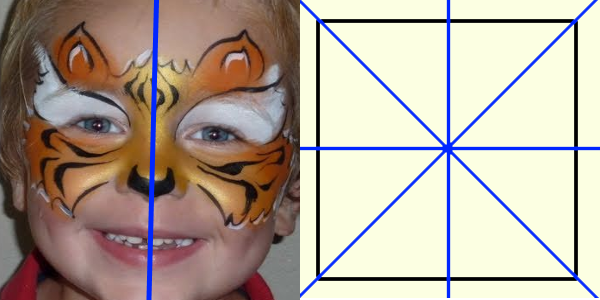
\includegraphics[width=0.9\columnwidth]{reflection}
\label{ref}
\caption{On the left, a face, exhibiting bilateral vertical reflection symmetry. On the right, a square, which contains four reflection axes. Reflection axes are marked with blue lines.}
\end{figure}

In two dimensional images, there are only four transformations that are not a simple composition of other transformations. These are \textit{reflection}, \textit{rotation}, \textit{glide reflection}, and \textit{translation}.

Reflection is the most well-known symmetry, with the vernacular for symmetry referring exclusively to it. It refers to when a line can be drawn on an image, and then every point on one side of the line has a corresponding point on the other side. The clearest examples of reflection symmetry in nature are probably the faces or bodies of animals. Reflection is often referred to by the number of reflection \textit{axes}, or lines, that the object contains. A face, for instance, would only contain one. A square, on the other hand, would contain three (See Figure~\ref{ref}).


Rotation is another very common example of symmetry in nature. Rotation refers to an object's ability to rotate around some center without changing. Rotation symmetry is generally referred to by the number of rotation angles that maintain this symmetry. For instance, a hexagon has 6-fold rotation symmetry, while a flower with six pedals would have 6-fold rotation symmetry (See Figure~\ref{rot})

\begin{figure}
\centering
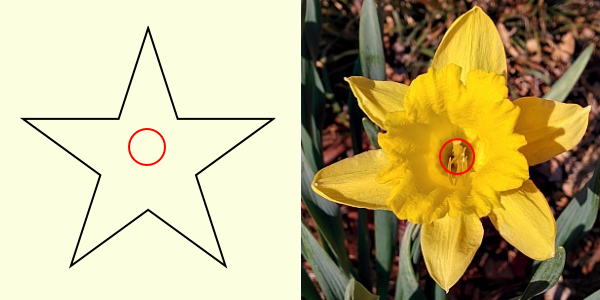
\includegraphics[width=0.9\columnwidth]{rotation}
\label{rot}
\caption{On the left, a flower exhibiting 6-fold rotation symmetry. On the right, a five-pointed star, exhibiting 5-fold rotation symmetry. Rotation centers are marked with a red circle}
\end{figure}

Translation symmetry refers to an object that repeats. For instance, in a brick wall, there are hundreds of bricks aligned in such a way that if you shifted the wall over by the length of exactly one brick, the wall would stay the same. Importantly, for this to make much sense in a mathematical sense, the wall would have to be infinitely long. Another example of translation symmetry would be a fence. If the fence was shifted by the length from one post to the next, the fence would stay the same. An important feature of translation symmetry is the \textit{tile}. The tile refers to the identical feature that is repeating. In the brick wall example, this is an individual brick, while in the fence post example, this is an individual fence post (See Figure~\ref{trans}).

\begin{figure}
\centering
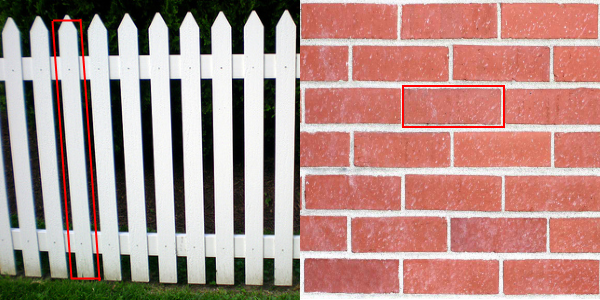
\includegraphics[width=0.9\columnwidth]{translation}
\label{trans}
\caption{On the left, a brick wall. On the right, a white fence. In both of these images, the image would have to repeat to truly exhibit translation symmetry. The tile is outlined in red.}
\end{figure}

The last basic symmetry is glide reflection. While reflection refers to something with a corresponding point directly across from it on the reflection axis, glide reflection refers to something that is reflected and then translated. The clearest examples of glide reflection in nature are footsteps. Each foot could be analyzed in terms of translation symmetry. However, halfway in between each footstep (the tile, in this case), there is a reflected footstep (made by the other foot). Thus, glide reflection is characterized by a "zig-zag" pattern of sorts, where the tile moves and reflects. Importantly, it is impossible to have glide reflection and reflection along the same axis. For instance, if someone walked some path and left footsteps that formed glide reflection, and then someone else walked along filling in a footstep that is a reflection of the original footstep, what would be left is just normal reflection, that happens twice as often as the glide reflection did (See Figure~\ref{glide}).

\begin{figure}
\centering
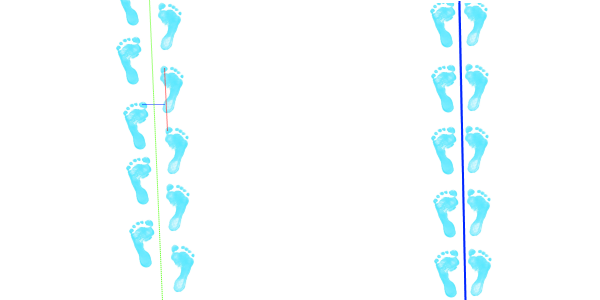
\includegraphics[width=0.9\columnwidth]{glide}
\label{glide}
\caption{On the left, footsteps exhibiting a glide reflection pattern. On the right, footsteps exhibiting a normal reflection pattern. Note that the two by definition cannot exist along the same axis.}
\end{figure}

In two dimensions, an infinitely large pattern that has translation symmetry is referred to as a \textit{wallpaper}. While all wallpapers have translational symmetry, they can still be divided based on their other symmetries, such as the axes they have reflection along. Interestingly, there are actually only seventeen real combinations of the set of symmetries \citep{wallpaper-proof}. Intuitively, this is because each tile must contain all of the other present symmetries then must also then fit together with an infinite number of tiles of the exact same type. 

\begin{figure}[!ht]
\centering
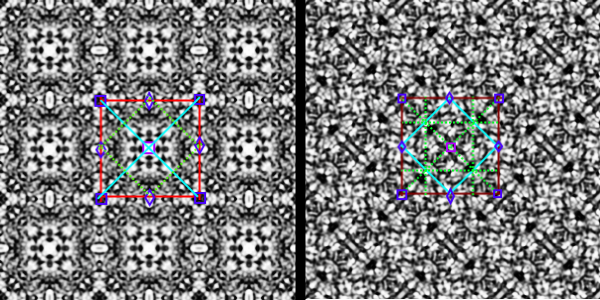
\includegraphics[width=0.9\columnwidth]{ann_images}
\label{P4GvP4M}
\caption{On the left is P4M, on the right is P4G. In each, one tile is marked with its symmetries. Notice that P4M has reflection axes on its tile border, whereas P4G does not.}
\end{figure}

Every wallpaper has some set of these symmetries, which we will also refer to as features. Each of the seventeen unique combinations are referred to as a wallpaper \textit{group}, with each wallpaper belonging to exactly one group. The symmetric features that define these groups consist of the basic symmetries we've discussed: rotation, reflection, glide reflection, and translation. Each wallpaper group has some set of these features. Among rotation, only 1-fold, 2-fold, 3-fold, 4-fold, and 6-fold tiles are possible. This is simply because other shapes of tiles cannot fit together in an infinite pattern. Table~\ref{sym-tab} gives a basic description of the seventeen groups as a set of their features. While this set has the majority of groups with a unique set of features, those with an equivalent set can be differentiated in other ways, such as what axes in the tile their reflection axes are along. See Figure~\ref{P4GvP4M} for an example. Importantly, any P4M or P4G would have the exact same tile annotations, even if their appearance was different.See Figure~\ref{P4MvP4M} for an example.



\begin{figure}[!ht]
\centering
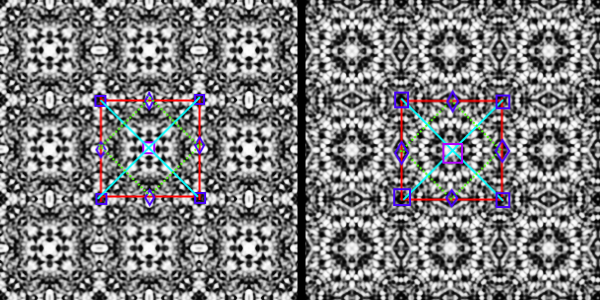
\includegraphics[width=0.9\columnwidth]{ann_images_same}
\label{P4MvP4M}
\caption{Both images are of the P4M group. Even though their appearance is quite different, they have the same symmetries in every single tile. }
\end{figure}

\begin{table}[!ht]
\centering
\resizebox{\columnwidth}{!}{%
\begin{tabular}{|l|c|c|c|c|c|c|c|c|c|}
\hline
Group & 2-fold & 3-fold & 4-fold & 6-fold & $T_1$ & $T_2$ & $D_1$ & $D_2$ &  tile \\ \hline
P1 & F & F & F & F & None & None & None & None & O \\ \hline
P2 & T & F & F & F & None & None & None & None & O \\ \hline
PM & F & F & F & F & Refl & None & None & None & Re \\ \hline
PG & F & F & F & F & Glide & None & None & None & Re \\ \hline
CM & F & F & F & F & None & None & Refl & None & Rh \\ \hline
PMM & T & F & F & F & Glide & Refl & None & None & Re \\ \hline
PMG & T & F & F & F & Glide & Refl & None & None & Re \\ \hline
PGG & T & F & F & F & Glide & Glide & None & None & Re \\ \hline
CMM & T & F & F & F & None & None & Refl & Refl & Rh \\ \hline
P4 & T & F & T & F & None & None& None & None & S \\ \hline
P4M & T & F & T & F & Refl & Refl & Refl & Refl & S \\ \hline
P4G & T & F & T & F & Glide & Glide & Refl & Refl & S \\ \hline
P3 & F & T & F & F & None & None & None & None & H \\ \hline
P3M1 & F & T & F & F & None & None & Refl& None & H \\ \hline
P31M & F & T & F & F & Refl & Refl & Refl & None & H \\ \hline
P6 & T & T & F & T & Refl & None & None & None & H \\ \hline
P6M & T & T & F & T & Refl & Refl & Refl & Refl & H \\ \hline
\end{tabular}%
}
\label{sym-tab}
\caption{Wallpaper groups represented as their symmetries. (Refl=Reflection, Glide=Glide Reflection, Re=Rectangular, Rh=Rhombic, O=Oblique, S=Square, H=Hexagonal)}
\end{table}

In representing wallpaper groups as a set of symmetries, we can then posit them in relation to each other. In this way, every group is either a subset or a superset of every other group.  If each group is placed with its relation to other groups, they form a graph, see Figure~\ref{graph}. If an arrow points from box $A$ toward box $B$, that means that $B$'s symmetries are subset of $A$'s symmetries.
\section{Prior Work}
Despite the age of the mathematical work on the topic, little has been done to connect these patterns to human perception. Symmetry beyond bilateral reflection has received little attention. This is perhaps due to work that suggests faces played a special role in our brain's evolution \citep{ffa}; bilateral reflection is the only symmetry they contain. There are several works covering bilateral reflection symmetry. \citet{bilateral-qual} explain that qualitative features are more important than quantitative differences in symmetry judgments. \citet{bilateral-color} discusses that having to check color increases the time it takes someone to determine whether an image is symmetric. They used this to argue that humans do not use color when making such judgments. 

However, \citet{bio} criticized these and other studies for relying on shapes that are not biological, which they claim is the origin of symmetry detection. Generally, many studies use blocks or other generated images rather than those of naturally occurring objects, such as faces or flowers. The authors further make the argument that bilateral vertical reflection is the only symmetry that has much prevalence in nature. While the examples provided should give some evidence of other types of symmetry in nature, we also seek to counter the claim that humans are not good at detecting other types of symmetry. 

The only study that we know of specifically dealing with wallpaper groups is \citet{clarke}. In that study, Clarke et al. found that subjects did not perform well in a symmetry group sorting task. Further, he found that they mostly used rotation in distinguishing among the groups. In this paper, we argue that the nature of Clarke's task was difficult for reasons other than perceiving the difference between two groups. Further, we argue that the strategy is not simply based on rotation.

\section{Research Questions}
Due to previous work not focusing on the role of symmetry groups in perception, we sought to design an experiment that tested which types of symmetry are easily perceived by humans. We also wanted to compare multiple theories of symmetry perception. In order to do this, we designed a task requiring people to differentiate wallpaper groups. Our research questions can be summarized as:

\begin{enumerate}
\item {\textbf{\textit{Can people naively distinguish among the wallpaper groups?}} In other words, without using any knowledge of symmetry, are they still able to see the differences? If the answer is yes, then we can expect that, at the very least, more features than reflection play a role in symmetry perception. Further, if people are very good at telling apart the wallpaper groups, then it is possible that group-theoretic symmetry actually plays a role in perception. This integrates well with a computational cognition paradigm.}
\item {\textbf{\textit{What features of symmetry drive the perception of symmetry?}} The presumption of previous studies is that reflection is the most important in perception, while Clarke's study claimed it was rotation. However, to the best of our knowledge, this is the first study to systematically isolate various symmetries. We will additionally investigate the role of the \textit{tile shape}}.
\end{enumerate}

\begin{figure}[!ht]
\centering
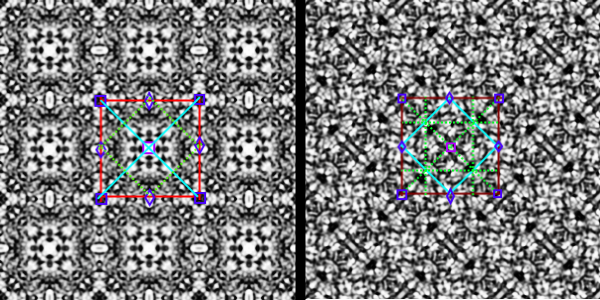
\includegraphics[width=0.9\columnwidth]{ann_images}
\caption{On the left is P4M, on the right is P4G. In each, one tile is marked with its symmetries. Notice that P4M has reflection axes on its tile border, whereas P4G does not.}
\label{fig:P4GvP4M}
\end{figure}

\begin{figure}[!ht]
\centering
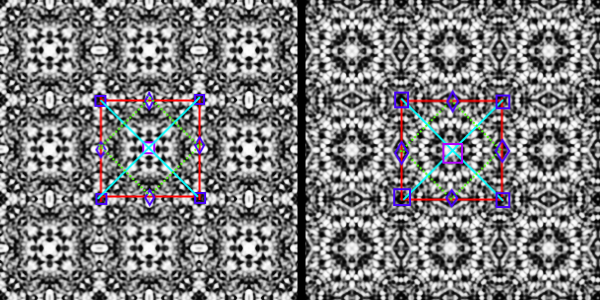
\includegraphics[width=0.9\columnwidth]{ann_images_same}
\caption{Both images are of the P4M group. Even though their appearance is quite different, they have the same symmetries in every single tile. }
\label{P4MvP4M}
\end{figure}
\section{Figures}

All artwork must be very dark for purposes of reproduction and should
not be hand drawn. Number figures sequentially, placing the figure
number and caption, in 10~point, after the figure with one line space
above the caption and one line space below it, as in
Figure~\ref{sample-figure}. If necessary, leave extra white space at
the bottom of the page to avoid splitting the figure and figure
caption. You may float figures to the top or bottom of a column, or
set wide figures across both columns.

\begin{figure}[ht]
\begin{center}
\fbox{CoGNiTiVe ScIeNcE}
\end{center}
\caption{This is a figure.} 
\label{sample-figure}
\end{figure}
\section{Analysis}
Our two basic research questions were addressed individually.

\subsection{Question 1}
To answer the first research question, we can rely on subjects' accuracy in distinguishing the two groups. We calculated this by combining the results for each as the distracter and the target. Then, we aggregated all the subjects and took the percentage that was correct. Our hypothesis was that participants can tell apart every group from every single group. To test this, we simply looked at the lowest percentage. We modeled the data as a binomial distribution with $\pi=0.5$, assuming the subjects were required to guess. Importantly, as there were $136$ tests of significance that took place, the chance of each one being significant at the $0.05$ level if they were on the edge of significance is $0.09\%$. 

In our study, the most difficult for participants was the distinction between “p4mm” and “pmm”. Across the 96 participants, only 56.8\% of trials were successful. On a single-tailed binomial distribution, there is a p-value of $0.06$ on that number of trials. While this misses the classical $0.05$ marker for significance, every single other group by group comparison meets it. Therefore, we find it likely that with more subjects, every group would have shown itself to be statistically distinguishable. The average accuracy fell right around 76.8\%, which is clearly far better than people would perform if they were at all guessing. Further, due to the number of significance tests, there would be some natural variation in any specific test.

\subsection{Question 2}
\textbf{This part I still need to do based on model comparison}
To answer our second question, we used a Linear Mixed Effects Regression model. Since we wanted to predict what caused the subjects to choose correctly, we used accuracy as the response variable. Thus, the first step was to change each task to its own record. Then, each feature we considered could have a positive of negative impact on the accuracy, represented as a slope.

Each task was boiled down to a comparison of the two symmetry group’s features. These features were whether or not the groups of the target and distracter images had the same tile shape, whether they both have reflection, whether they both have glide reflection, and whether they have the same rotation order. Lastly, we also included the value for the shortest path on the subgroup relation graph; for instance, the distance from “p6m” to “p6” is 1. While each of the first four refer to some basic feature of symmetry, the graph distance is included as somewhat of an alternative theory. In short, it would posit that humans perceive symmetry very closely to its mathematical analysis, instead of as a collection of individual symmetries.

We used two random effect variables, which represent uncontrolled aspects of the model. The first is the actual participant who performed the task, which obviously has some effect on the accuracy. The second is the actual images they looked at: each participant was presented a different combination of the 85 total images we used. Thus, the combination they looked at could also play a role, even if each image was from the same group.

\begin{figure}[!ht]
\centering
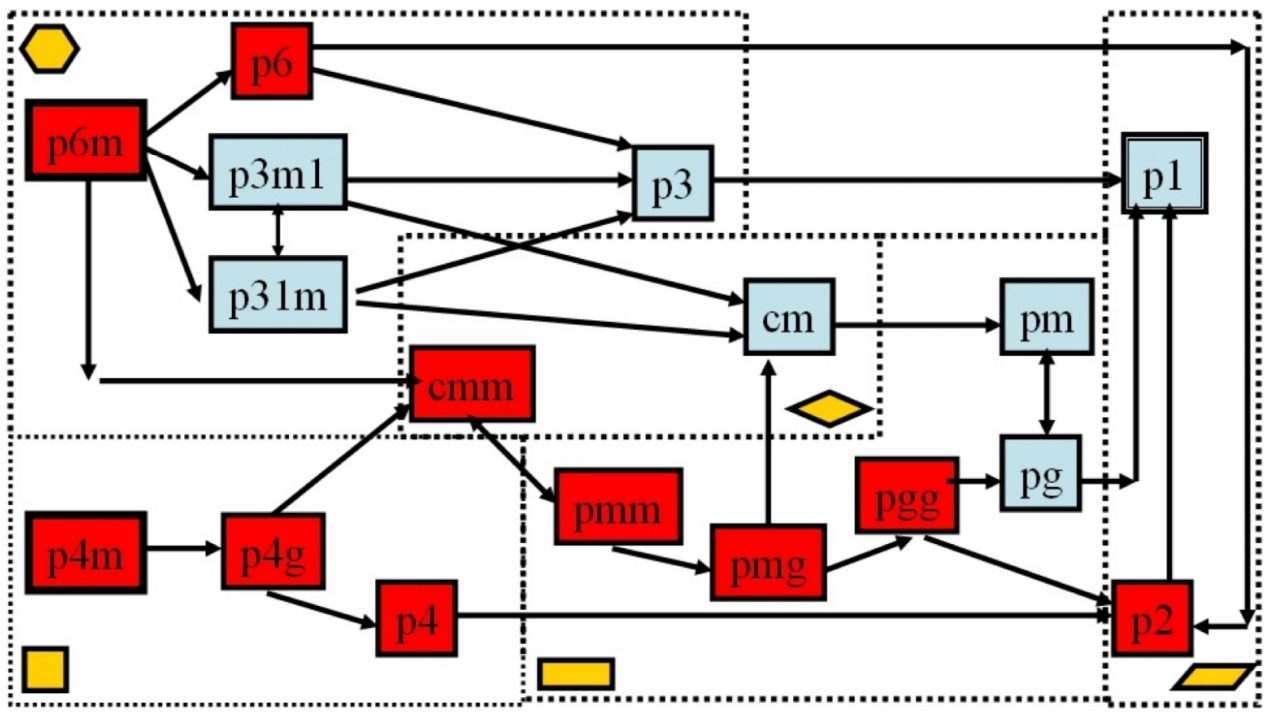
\includegraphics[width=0.9\columnwidth]{Yanxi_Graph}
\label{graph}
\caption{The subgroup relation graph}
\end{figure}

No interaction terms were considered, so the equation was simply: 

\[\mathrm{acc} \sim \mathrm{rot}+\mathrm{ref}+\mathrm{gref}+\mathrm{tile}+\mathrm{distance}+(1\mid \mathrm{subject})+(1 \mid \mathrm{task})\]

To be clear, accuracy (acc) in each record was 1 or 0. Rotation (rot), reflection (ref), glide reflection (gref), and tile shape (tile) were all either true or false based on whether the target image had the same value as the distracter image. The subject and the task were numeric based on their ID in the database. Please see Table~\ref{results} for a break-down of the results.

This shows that tile shape, glide reflection, and distance were all significant in determining accuracy. However, neither reflection or rotation are.

\begin{table}
\centering
\begin{tabular}{|l|ccc|}
\hline
& Estimate & Std. Error & t value \\ \hline
Rotation& 0.005650& 0.007742& 0.73 \\ \hline
Reflection& -0.004545& 0.005768& -0.79 \\ \hline
Glide Reflection& 0.06854& 0.005382& 3.13* \\ \hline
Tile& -0.030277& 0.006732& -3.87* \\ \hline 
Distance& 0.028984& 0.002781& 10.42* \\ \hline
\end{tabular}
\label{results}
\caption{Fixed Effects}
\end{table}
\section{Discussion}
There are several results that we obtained that require some explanation in order to sit neatly on top of the existing literature. \citet{clarke} found that people aren't very good at the task, but that the strategy they use tends to rely on rotation. However, Clarke's study relies on grouping images together. When presented with this task, it seems unlikely that most people would immediately choose to use 17 groups. Indeed, the number of sets participants made varied wildly in Clarke?s study, from 2 to 23 \citep{clarke}. This makes it somewhat difficult to analyze the actual strategy participants used. Further, if people are to choose some number of groups less than 17, rotation may be a logical method to sort them by. Importantly, Clarke's task does not isolate perception very well. It allows participants an unlimited amount of time, allowing them to use other sorts of analytical reasoning. Second, due to working memory constraints, it would be difficult for participants to recall precisely what type of image corresponded to each bin as they continued to sort. These confounds could explain the difference.

\begin{table}
\centering
\begin{tabular}{|l|cccc|}
\hline
& Estimate & Std. Error & z value & Pr(<|z|)  \\ \hline
(Intercept) & 0.95971 &  0.09950 & 9.645 & <2e-16*** \\ \hline
T1 & -0.24795 &  0.04150 & -5.975 & 2.30e-09*** \\ \hline
T2 & -0.07746 & 0.04026 & -1.924 & 0.0544 \\ \hline
D1 & -0.31416 & 0.04063 & -7.732 & 1.06e-14*** \\ \hline
D2 & 0.10197 & 0.04431 & 2.301 & 0.0214* \\ \hline
2fold & 0.01214 & 0.03540 & 0.343 & 0.7316 \\ \hline
3fold & -0.18056 & 0.04197 & -4.302 & 1.69e-05*** \\ \hline
4fold & 0.32353 & 0.04282 & 7.555 & 4.19e-14*** \\ \hline
6fold & -0.07538 & 0.04484 & -1.711 & 0.0870 \\ \hline
tile & -0.07891 & 0.05556 & -1.420 & 0.1555 \\ \hline
distance & 0.22420 & 0.01872 & 11.978 & <2e-16*** \\ \hline
\end{tabular}
\label{fixeff}
\caption{Fixed Effects}
\end{table}

In general, this paper advocates for a model of symmetry/pattern detection that is mathematically driven. We believe the subgroup distance to be one method for capturing the method humans perceive regularities. Importantly, it is not the only one and it may not even be the best one. By using Dijkstra's algorithm, we weighted each edge to be exactly equal. However, that's not necessarily the case. While "p1" and "p2" differ by exactly one symmetry (the 2-fold rotation), "p2" and "pgg" differ by three symmetries. Another possible view is to calculate the distance using the Hamming distance between each pair, rather than the relation graph. However, there are clearly multiple definitions of even the same mathematical model when it is operationalized for perception, which complicates the story.

As the model containing only subgroup distance outperformed the other simple models, we find it likely that subgroup distance is the single most useful feature. However, it should be clear from our results displayed earlier that distance alone does not tell the whole story. Thus, we interpret the additional features in the converged model as having an overly important role in the process of pattern recognition. In other words, human perception might use some quick heuristics involving these symmetries instead of doing a full analysis. 

\begin{table}
\centering
\resizebox{\columnwidth}{!}{%
\begin{tabular}{|l|cccccccccc|}
\hline
(Intercept) & T1 & T2 & D1 & D2 & 2fold & 3fold & 4fold & 6fold & tile & distance  \\ \hline
T1 & -0.191 &   & & & & & & & & \\ \hline
T2 & -0.090 & -0.556 &  & & & & & & &  \\ \hline
D1 & -0.216 & 0.111 & 0.040 & & & & & & & \\ \hline
D2 & -0.051 & -0.005 & -0.137 & -0.572 & & & & & & \\ \hline
2fold & -0.472 & 0.113 & -0.010 & 0.136 & -0.061 & & & & & \\ \hline
3fold & -0.127 & 0.148 & -0.090 & 0.088 & 0.039 & -0.068 & & & & \\ \hline
4fold & -0.464 & 0.179 & -0.121 & 0.172 & -0.245 & 0.160 & 0.237 & & &  \\ \hline
6fold & -0.245 & 0.001 & 0.048 & 0.055 & -0.192 & 0.060 & -0.413 & 0.029 & & \\ \hline
tile & -0.169 & -0.210 & 0.241 & -0.141 & 0.072 & 0.180 & -0.525 & -0.292 & 0.189 & \\ \hline
distance & -0.713 & 0.052 & 0.082 & 0.046 & 0.116 & 0.405 & -0.029 & 0.296 & -0.026 & 0.350 \\ \hline
\end{tabular}%
}
\label{corr}
\caption{Correlation of Fixed Effects (note that this is the empirical correlation rather than the analytical relationship)}
\end{table}

For instance, why are $T_1$ and $D_1$ significant (the vertical and positive diagonal axis), but not $T_2$ and $D_2$ (the horizontal and negative diagonal axis)? While it seems easy to attribute it to perception, it is important to realize there are substantial correlations among features in the wallpaper groups. In some cases, this should be obvious: if a wallpaper group has 6-fold rotation, it is guaranteed to have both 2-fold rotation and 3-fold rotation by the definition. In the case of the reflection axes, there are substantial correlations (about $0.5$) between $D_1$ and $D_2$ and between $T_1$ and $T_2$. Thus, while it's somewhat difficult to disentangle their independent effects, it seems clear that both $T_1$ and $D_1$ are at least more important, as the models including them instead of $T_2$ and $D_2$ perform better on the earlier discussed metrics. However, $D_2$ is also a significant predictor even considering $D_1$, while $T_2$ is not a significant predictor while considering $T_1$. A possible explanation for this could result in faces, with $D_1$ and $D_2$ representing faces at an angle. As mentioned earlier, there are some biological reasons for believing humans are adept at recognizing faces \cite{ffa}.     

The overabundance of the role of reflection symmetry in the literature could be due to the lack of knowledge of researchers of other types of symmetry. Further, it could be related to vast literature on faces, which contains reflection symmetry but lacks all other types. While our results show that people obviously can detect reflection symmetry, it does not tell the whole story.

In the case of rotation, the most significant features were 3-fold and 4-fold. Interestingly, the effect of 4-fold rotation is positive (if both groups both have 4-fold rotation or both don't, accuracy improves), while the effect of 3-fold rotation is negative. This means that groups with 4-fold rotation are not necessarily easy to determine from groups without it, but they are easy to tell apart internally. This is very possibly due to 4-fold rotation's correlation with the other features.

For 3-fold rotation, it is possible that (unlike 4-fold rotation), it plays a more significant role due to its lack of ubiquity. Many objects humans interact with in the modern world contain 4-fold rotation, to the point where perhaps it is so common that it is no longer a useful heuristic. On the other hand, 3-fold rotation is a bit more rare, and thus may have some special significance.

Lastly, the highly significant effect of distance is interesting. The simplest reading of this is that people perceive group to group similarity as more than any individual feature. Computer vision has long been inspired by wallpaper groups \citep{yanxi1}\citep{yanxi2}, and this result lends further credence to the idea that they are some fundamental part of human perception.
\section{Conclusion}
This paper argues that human pattern perception is sensitive to more types of symmetry than previously thought. To date, data on types of symmetry other than bilateral reflection were limited; however, we present evidence that humans can and do perceive the other types of symmetry. We found that all but one pair of wallpaper groups are reliably distinguishable ($p < 0.05$) and all are likely distinguishable ($p < 0.1$). After comparing models, we found that certain axes in reflection and certain types of rotation both play a role in symmetry detection. Notably, we also found that subgroup distance is a viable predictor of the accuracy of similarity judgments.
\bibliographystyle{elsarticle}
\section*{References} %temp?, not sure what's wrong
\bibliography{symmetry,symmetry2,perception,yanxibook,statistics,statistics2,statistics3}

%\bibliography{perception}

\end{document}

\endinput
%%
%% End of file `elsarticle-template-harv.tex'.
